% !TEX program = pdflatex
\documentclass{article}
\usepackage{tikz}
\usetikzlibrary{positioning,arrows.meta,shapes.geometric,calc}
\begin{document}
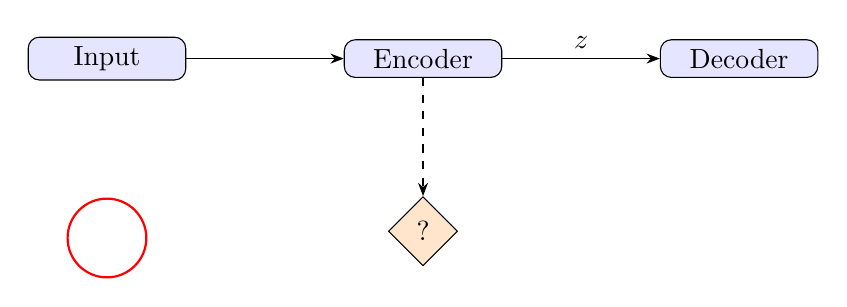
\begin{tikzpicture}[node distance=1.5cm and 2cm, box/.style={draw,rounded corners,fill=blue!10,minimum width=2cm}]
\node[box] (in) {Input};
\node[box,right=of in] (enc) {Encoder};
\node[box,right=of enc] (dec) {Decoder};
\node[diamond,draw,fill=orange!20,below=of enc] (d) {?};
\draw[-{Stealth}] (in) -- (enc);
\draw[-{Stealth}] (enc) -- node[above]{$z$} (dec);
\draw[-{Stealth},dashed] (enc) -- (d);
\draw[red,thick] ($(in.south)+(0,-2)$) circle (0.5);
\end{tikzpicture}
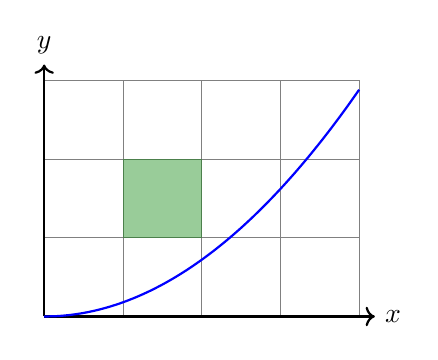
\begin{tikzpicture}
\draw[help lines] (0,0) grid (4,3);
\draw[thick,->] (0,0) -- (4.2,0) node[right]{$x$};
\draw[thick,->] (0,0) -- (0,3.2) node[above]{$y$};
\draw[domain=0:4,smooth,variable=\x,blue,thick] plot ({\x},{0.18*\x*\x});
\fill[green!50!black,opacity=.4] (1,1) rectangle (2,2);
\end{tikzpicture}
\end{document}
